\chapter{Systemdesign} % (fold)
\label{sec:systemdesign}
Innerhalb dieses Abschnitt sollen die konkreten Technologien beschrieben werden, die gewählt wurden um ein System zu entwickeln welches für Latentztests verwendet werden kann.
\section{Datenbankdesign} % (fold)
Für die Durchführung des Experiments werden zwei Datenbanktypen verwendet, welche nachfolgend mit ihrer konkreten Konfiguration beschrieben werden. In jeder Datenbank sind 5000 Personen als auch Issue Objekte vorhanden, sowie 2500 Project Objekte, somit enthählt jede Datenbank 12500 Datensätze.
\label{sec:datenbankdesign}
\subsection{Relationales Datenbankdesign} % (fold)
\label{sec:relationalesdatenbankdesign}

\begin{figure}[H]
	\centering
	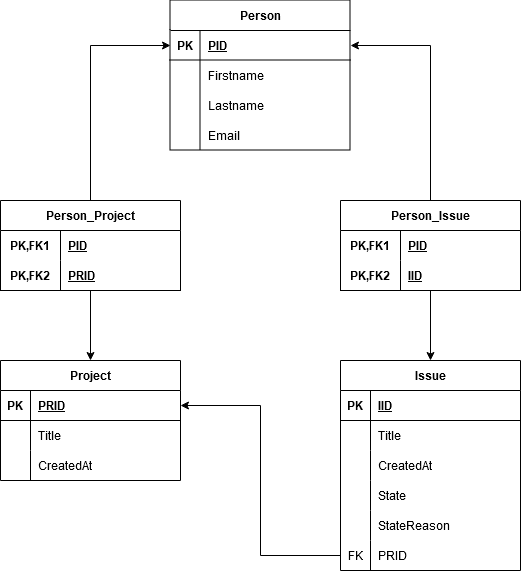
\includegraphics[scale=0.6]{Illustrations/table_diagram.png}
	\caption{Tabellen Diagramm}
\end{figure}
Um eine realtionale Datenbank aus dem gegebenen Datenmodell (Abb.3) zu erstellen muss dieses wie in Abb. 4 zu sehen ist angepasst werden, um die Beziehung zwischen Person und Projekt als auch Person und Issue abzubilden. Somit ergeben sich für die relationale Datenbank fünf Tabellen welche in einer PostgreSQL Datenbank realisiert werden. PostgreSQL wird verwendet, da es ein leistungsfähiges, objekt-relationales Datenbanksystem bietet welches Open-Source ist und dadurch kostenfrei zur Verfügung steht. 
% subsection relationalesdatenbankdesign (end)
\subsection{Graphdatenbankdesign} % (fold)
\label{sec:graphsdatenbankdesign}
Um eine Graphdatenbank zu erstellen benötigt man keine definierten Tabellen, da diese die Daten schemafrei speichert. Die Nodes werden bei der Erstellung entsprechend der Objekte benannt, ebenso werden die Beziehungen zwischen den Nodes bei der Erstellung benannt. Als Graphdatenbank wird auf neo4j zurückgegriffen. Es ist eine der am weitesten verbreiteten Graphdatenbanken und bietet eine hohe Benutzerfreundlichkeit. In Abbildung 5 ist eine Demonstration einer Beziehung zwischen jeweils einem Node zu sehen. Die Kanten sind als gerichtete Kanten abgebildet, dabei hat Person zwei ausgehende Kanten, Projekt zwei eingehende und Issue jeweils eine eingehende als auch eine ausgehende Kante. 


\begin{figure}[H]
	\centering
	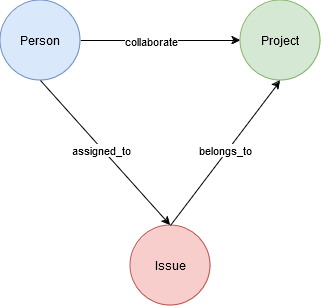
\includegraphics[scale=.8]{Illustrations/graph_diagram}
	\caption{Graph Diagramm}
\end{figure}
% subsection graphdatenbankdesign (end)

% section datenbankdesign (end)

\section{Schnittstellendesign} % (fold)
\label{sec:schnittstellendesign}

\subsection{REST}
\label{sec:rest}
Bei REST wird für jedes Testszenario ein seperater Endpunkt benötigt. Hierbei wurden vier verschiedene Endpunkte mit unterschiedlichen Komplexität entworfen.
\begin{itemize}
\item \textbf{GET api/persons/:pid}: Dieser Endpunkt ermöglicht das Abrufen einer bestimmten Person anhand ihrer ID. Die API liefert dabei ein JSON-Objekt zurück, dass die Person mit den Attributen Vorname, Nachname und E-Mail-Adresse beschreibt und wie folgt strukturiert ist.
\begin{center}
\begin{BVerbatim}
{
    "pid": 10,
    "firstname": "Cecilla",
    "lastname": "Beningfield",
    "email": "cbeningfield9@wp.com"
}
\end{BVerbatim}
\end{center}

\item Mit dem Endpunkt  \textbf{GET api/persons} können alle in der Datenbank gespeicherten Personen abgerufen werden. Die Antwort umfasst 5000 Personenobjekte im JSON-Format.
\begin{center}
\begin{BVerbatim}
[
    {
        "pid": 1,
        "firstname": "Ruby",
        "lastname": "Burchatt",
        "email": "rburchatt0@msn.com"
    },
	[...]
    {
        "pid": 5000,
        "firstname": "Murdoch",
        "lastname": "Simonitto",
        "email": "msimonittorr@google.ca"
    }
]
\end{BVerbatim}
\end{center}
\item Der Endpunkt \textbf{GET api/persons/:pid/projects/issue} erhöht die Komplexität, da hier nicht nur auf eine einzelnes Objekt zugegriffen wird. Stattdessen erfordert die Abfrage mehrere Objekte, die miteinander in Abhängigkeit stehen, um die Anfrage zu bearbeiten. Die Antwort wird in folgendem Format erwartet:
\begin{center}
\begin{BVerbatim}
[
   {
        "iid": 1,
        "title": "Pixope",
        "createdAt": "2024-07-23 00:00:00",
        "state": "Closed"
        "stateReason": "Cancelled"
    },
    {
        "iid": 2876,
        "title": "Zoomlounge",
        "createdAt": "2020-08-26 00:00:00",
        "state": "Open"
        "stateReason": "Bug"
    },
]
\end{BVerbatim}
\end{center}

\item \textbf{POST api/persons/:pid/projects/:prid/issues}: Dieser Endpunkt ermöglicht das Erstellen eines neuen Issues in der Datenbank, um nicht nur Abfragen zu testen, sondern auch das Hinzufügen von Daten. Im Body der Anfrage wird ein Issue-Objekt im JSON-Format übergeben. 
\begin{center}
\begin{BVerbatim}
{
    "title":"test",
    "createdAt":"2023-02-21T00:00:00",
    "state":"Open",
    "stateReason":"Bug"
}
\end{BVerbatim}
\end{center}
Die Antwort enthält das erstellte Issue-Objekt, das eine gültige ID sowie Verknüpfungen zu dem zugehörigen Projekt und der Person beinhaltet.
\begin{center}
\begin{BVerbatim}
{
    "iid": 5207,
    "title": "test",
    "createdAt": "2023-02-21T00:00:00",
    "state": "Open",
    "stateReason": "Bug",
    "project": {
        "prid": 12,
        "title": "Y-find",
        "createdAt": "2021-01-10T00:00:00"
    },
    "assignee"{
        "pid": 1,
        "firstname": "Ruby",
        "lastname": "Burchatt",
        "email": "rburchatt0@msn.com"
    },
}
\end{BVerbatim}
\end{center}

\end{itemize}

% section rest (end)

\subsection{GraphQL}
GraphQL nutzt nur einen Enpunkt, nämlich api/graphql die Anfragen werden im Body mithilfe der GraphQL Query Language definiert. Nachfolgend werden die 4 Anfragen beschrieben, die den in 5.2.1 aufgelisteten REST-Endpunkten enstprechen.

\begin{center}
\begin{BVerbatim}
query{
    person(id : 10){
	pid
	firstname
	lastname
	email
    }
}
\end{BVerbatim}
\end{center}


\begin{center}
\begin{BVerbatim}
query {
    persons {
        pid
        firstname
        lastname
        email
    }
}
\end{BVerbatim}
\end{center}


\begin{center}
\begin{BVerbatim}
query{
    person(id : 10){
        projects{
	    issues{
		iid
		title
		createdAt
		state
		stateReason
	    }
        }
    }
}
\end{BVerbatim}
\end{center}


\begin{center}
\begin{BVerbatim}
mutation{
    createIssue(input:{
	title : „Bug in Login“
	createdAt : „2024-12-03T12:30:00
	state : „Open“
	stateReason : „Error in Login“
	prid: 80
	}){
	iid
	title
	state
	stateReason
	createdAt
    }
}
\end{BVerbatim}
\end{center}


\label{sec:graphql}
% section graphql (end)

\subsection{Datenbank}
\label{sec:datenbank}
% section datenbank (end)


% section schnittstellendesign (end)
\section{Testumgebung} % (fold)
\label{sec:testumgebung}
Zur Ermittlung der Latenzzeiten werden API-Abfragen durchgeführt, bei denen die Antwortzeiten in Millisekunden protokolliert werden. Dafür wird eine Testumgebung mit zwei unterschiedlichen Endgeräten benötigt, um die Last auf mehrere Geräte zu verteilen. Die APIs laufen auf einem Server in Frankfurt, der mit 4 Kernen, 24 GB Arbeitsspeicher, einer 1 Gbit-Internetverbindung und Ubuntu 22.04 als Betriebssystem ausgestattet ist.
Die Abfragen erfolgen von einem PC mit 8 Kernen, 32 GB Arbeitsspeicher, einer 50 Mbit-Internetverbindung und Windows 10 als Betriebssystem. Die durchschnittliche Latenz (Ping) zwischen Server und PC beträgt 24 ms. Um Schwankungen in der Netzwerkauslastung und der Systembelastung zu minimieren, werden pro Testszenario und API jeweils 100 Anfragen ausgeführt. Insgesamt ergibt dies bei 4 APIs und 4 Testszenarien eine Datengrundlage von 1600 Latenzzeiten.


% section testumgebung (end)


% chapter Systemdesign (end)